\documentclass[journal,12pt,twocolumn]{IEEEtran}
\usepackage{amsmath,amssymb,amsfonts,amsthm}
\usepackage{txfonts}
\usepackage{tkz-euclide}
\usepackage{listings}
\usepackage{gvv}
\usepackage[latin1]{inputenc}
\usepackage{array}
\usepackage{pgf}
\usepackage{lmodern}

\begin{document}
\bibliographystyle{IEEEtran}

\vspace{3cm}

\title{}
\author{EE23BTECH11024 - G.Karthik Yadav$^{*}$
}
\maketitle
\newpage
\bigskip

% \renewcommand{\thefigure}{\theenumi}
% \renewcommand{\thetable}{\theenumi}


\section*{Exercise 9.1}

\noindent 1. \hspace{2pt}Write the first five terms of the sequence\\
$a_n = n \brak{n+2}$

\solution

\setlength{\arrayrulewidth}{0.2mm}
\setlength{\tabcolsep}{15pt}
\renewcommand{\arraystretch}{1.15}


\begin{table}[ht]
  \centering
  \begin{tabular}{|c|c|c|}
    \hline
    	Symbol & Parameters & value\\
    \hline
	  $u\brak{n}$ & unit step function &  \\
    \hline
	  $x\brak{n}$ & general term of the series & $\brak{n+1}\brak{n+3}u\brak{n}$ \\
    \hline 
	 $X\brak{z}$ & Z-transform of x(n) & ? \\
    \hline
  \end{tabular}
  \vspace{0.3cm}
  \caption{Input Parameters}
  \label{tab:1.11.9.1.1}
\end{table}

\begin{align}
u\brak{n} & \xrightarrow {Z} \frac{1}{\brak{1-z^{-1}}} ,   \abs{z} >1 \label{eq:24.11.9.1.1.1}\\
    n u\brak{n} & \xrightarrow {Z} \frac{z^{-1}}{\brak{1-z^{-1}}^2} ,   \abs{z} >1 \label{eq:24.11.9.1.1.2}\\
    n^2 u\brak{n} & \xrightarrow{Z} \frac{z^{-1}\brak{z^{-1}+1}}{\brak{1-z^{-1}}^3} ,  \abs{z} > 1\label{eq:24.11.9.1.1.3}
\end{align} 


\begin{align}
    X \brak{z} & = \sum_{n=-\infty}^{\infty}  \brak{n+1}\brak{n+3} u \brak{n}   z^{-n} \\
    & = \sum_{n=-\infty}^{\infty}  \brak{n^{2}u\brak{n} + 4 n\, u\brak{n}  + 3u\brak{n} } z^{-n}
\end{align}    

Using eq \eqref{eq:24.11.9.1.1.1} , eq \eqref{eq:24.11.9.1.1.2} and eq \eqref{eq:24.11.9.1.1.3}
\begin{align}
     X \brak{z} & = \frac{ 3-z^{-1}}{\brak{1-z^{-1}}^3} \text{ ,}\qquad \abs{z}>1
\end{align}

\begin{figure}[ht]
   \centering
   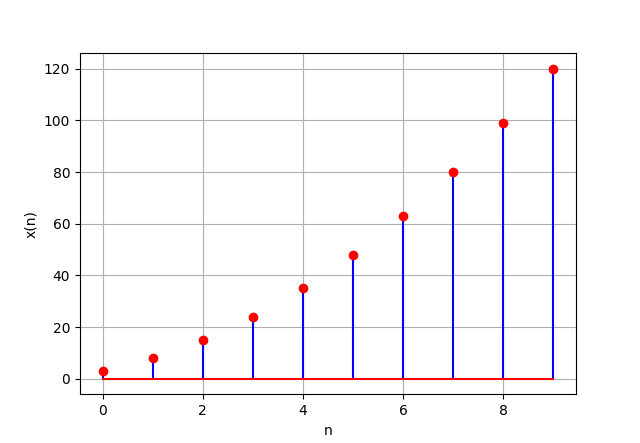
\includegraphics[width=1\columnwidth]{figs/plot1.png}
   \caption{Plot of x(n) vs n}
   \label{fig: 1.11.9.1.1}
\end{figure}


\end{document}
